\documentclass[11pt,a4paper]{article}
\usepackage[paper=a4paper,margin=1in]{geometry}% 


\usepackage[utf8]{inputenc}
\usepackage{graphicx}
\graphicspath{ {./images/} }
\usepackage{xcolor}

\usepackage{hyperref}
\hypersetup{
    colorlinks=true,
    linkcolor=blue,
    filecolor=magenta,      
    urlcolor=cyan,
    citecolor=blue
}


\usepackage{booktabs}
\usepackage{array}
\newcolumntype{R}[1]{>{\raggedright\let\newline\\\arraybackslash\hspace{0pt}}m{#1}}

\usepackage{lscape}

\usepackage{url} 

\usepackage{titlesec} % for spacing around headings
\titlespacing\subsection{0pt}{5pt}{0pt} % left, before, after
\setlength{\parindent}{0pt}
\setlength{\parskip}{0.5em}


% If we want to remove section numbering then this works
\setcounter{secnumdepth}{0}


\usepackage[framemethod=default]{mdframed}

% coloured border to distinguish manual for each block (Sarah mentioned doing something like this)

\usepackage{xcolor}
\usepackage{eso-pic}

\definecolor{border}{RGB}{112,191,68}


\newdimen\extraxsep
\newdimen\extraysep
\extraxsep=20mm
\extraysep=20mm
\newcommand\frameattext[3]{%
  \linethickness{#3}%
  \AddToShipoutPicture*{%
    \AtTextLowerLeft{%%text-boder
       \put(\LenToUnit{-,5\extraxsep},\LenToUnit{-0.5\extraysep}){\color{#1}%
             \rule{\dimexpr\textwidth+\extraxsep\relax}{\dimexpr\textheight+\extraysep\relax}}%
       \put(\LenToUnit{-,5\extraxsep},\LenToUnit{-0.5\extraysep}){\color{#2}%
       \framebox(\LenToUnit{\dimexpr\textwidth+\extraxsep\relax},%
                 \LenToUnit{\dimexpr\textheight+\extraysep\relax}){}
       }
    }%
  }%
}

%\input{aretefactdef.tex}



\begin{document}



\begin{titlepage}
	{\centering
	 
\includegraphics[width=0.3\linewidth]{images/UOY-Logo-Stacked-shield-PMS432-2.png}\par\vspace{1cm}
 	{\Large{Title of your research project
 	}}\par\vspace{1cm}
% {\large{Software Platform}}\par{\vspace{1cm}}
% {PO number DSTLX-1000117326}\par {Report date: 31 May 2018} \par\vspace{1cm}
Your Name. \par \vspace{0.5cm}
Progression Report Year ??\\

%Copyright \textcopyright~ University of York (optional)\par
\par \vspace{5cm}
\textbf{4th October 2023} 
\par\vspace{5mm}
}

\centering 
\textsf{Contact : emailaddress@york.ac.uk.}\par \vspace{1cm}
%\textsf{(Any commercial in confidence statement) (optional)} \par\vspace{0.5cm}
%\textsf{Classification if appropriate}

\end{titlepage}


\section*{Abstract}

This template provides guidelines to what should go in your progression report. Please note, you are producing your report for your internal assessor and supervisor(s) and should therefore be writing your content with them in mind as your audience. It is not being written for a lay person, or your PGR peers.

\tableofcontents
\newpage
\section{Introduction/Direction of Research}

Provide an overview of the problem you are tackling, motivate why it is interesting/important, and describe the research questions you will address in order to tackle it.  Typically 1-4 pages, typically 2-5 research questions.  (Avoid “closed” questions with yes/no answers.)

\section{Literature review/Field of Knowledge}
For \textbf{\emph{CS PhD researchers}} only - please provide the following for the progression report in the specified year of study:
\begin{itemize}
    \item 1st Year : An in-depth academic review and critique of the research context, placing your problem in context, typically 15-30 pages, with 50-150 references.  If your topic covers several disciplines, you will need a sufficient review of each to establish the context.
    \item 2nd Year : Any additional material from your continued reading of the literature, plus any new areas that have become prominent, typically 1-10 pages, with 10-50 references
\end{itemize}

Where appropriate references can be added to the references.bib file and cired as follows~\cite{Kelly_97}.

For \textbf{\emph{IGGI PhD researchers}} only - please provide the following for the progression report in the specified year of study:
\begin{itemize}
    \item 1st Year : Demonstrate sufficient acquaintance with the relevant field of knowledge to place your research into context by providing a summary of the area of research and key papers that articulate the state of research, typically 3-10 pages with 20-50 references.
    \item 2nd Year : An in-depth academic review and critique of the research context, placing your problem in context, typically 15-30 pages, with 50-150 references.  If your topic covers several disciplines, you will need a sufficient review of each to establish the context.
    \item 3rd Year : Any additional material from your continued reading of the literature, plus any new areas that have become prominent, typically 1-10 pages, with 10-50 references
\end{itemize}

\section{Research Methods}
Discuss how you will conduct your research: what research method(s), tools, and techniques you will use, and why these are the appropriate ones to address your research questions (this could be any of, mathematical proofs, software development, hardware development, user experiments, field trials, statistical analyses, or other methods)

Discuss your current capability to use your proposed method(s), and any training needed to fill the gaps.

Typically 1-2 pages

\section{Preliminary results/Progress to date}

For \textbf{\emph{CS PhD researchers}} only - please provide the following for the progression report in the specified year of study:
\begin{itemize}
    \item Year 1 : optional. Typically 0-10 pages
    \item Year 2 : Details of research progress to date. Typically a published or ready to submit paper, attached to the submission; otherwise similar details provided in the report body
\end{itemize}

For \textbf{\emph{IGGI PhD}} researchers only - please provide the following for the progression report in the specified year of study:
\begin{itemize}
    \item Year 1 : optional. Typically 0-10 pages
    \item Year 2 : Details of research progress to date, typically 5-10 pages. A published or ready to submit paper of publishable quality should be attached to the submission in either year 2 or year 3 (depending on status of knowledge exchange).
    \item Year 3 : Details of research progress to date, typically 5-10 pages. Your published or ready to submit paper of publishable quality should be attached to the submission in year 3 even if it was submitted in year 2.
\end{itemize}

\section{Planning}
\begin{itemize}
    \item Your plan for the next year of study, broken down into tasks, including a timeline figure of when the tasks will be tackled (a gantt chart is recommended as shown in Figure~\ref{fig:Gantt})
    \item A table of risks, with their likelihood / severity / mitigation (include technical risks as shown in Table~\ref{tab:Risks})
\end{itemize}

\begin{table}[h]
\begin{center}
    \caption{Risk table.\label{tab:Risks}}
    \begin{tabular}{R{4.0cm}R{2.0cm}R{2.0cm}R{4.0cm}}\toprule
    Risk & Likelihood & Severity & Counter-measure(s) \\ \midrule
    1. First risk & low, medium, high& low, medium, high& 1. Mitigation \newline 2. Mitigation\\ \midrule
    2. Second risk & low, medium, high& low, medium, high& 1. Mitigation \newline 2. Mitigation\\ \bottomrule
    \end{tabular}
\end{center}
\end{table}
\section{Training completed}

\begin{itemize}
    \item Brief overview and evidence that the mandatory CS training has been completed (eg, attach screenshots from the VLE to the submission)
    \item Short discussion of any other training that has been completed
    \item (IGGI 1st year only) Brief overview and evidence of IGGI modules completed (e.g. attach screenshots from the VLE to the submission)
    \item (IGGI only years 1,2,3) brief summary of participation at IGGI conference, Global Game Jams, other IGGI events, etc 
\end{itemize}

\section{Knowledge Exchange (KE) \& Impact (IGGI only)}
\begin{itemize}
    \item IGGI Year 2 or Year 3 - Brief overview and provide evidence of completed KE activity (attach KE reports to this submission)
    \item Brief summary of any ongoing KE and impact related activities
    \item Your evidence of completed KE activity (i.e. attached KE reports) should be included in your Year 3 report even if it was included in Year 2. 
\end{itemize}

\section{Ethics (including Data Management)}
\begin{itemize}
    \item your conduct of the research 
    \item ethical considerations for  any experiments you plan to perform, if applicable. Please note any research involving human participants or human data will need to apply for ethical approval beforehand. 
    \item ethical implications of data you collect, if applicable. If you do not think there are any ethical implications, then you will need to explain why this is the case. 
    \item data and code management plan 
\end{itemize}



\section{Responsible Research \& Innovation}
Reflect on how your past and proposed future research, including how you disseminate it, maximises the positive impact it can make by appropriately considering:
\begin{itemize}
    \item equality, diversity, and inclusion, 
    \item is your research ethically responsible 
    \item how your research is designed to meet the needs of stakeholder groups . 
\end{itemize}




\begin{landscape}
\begin{figure}
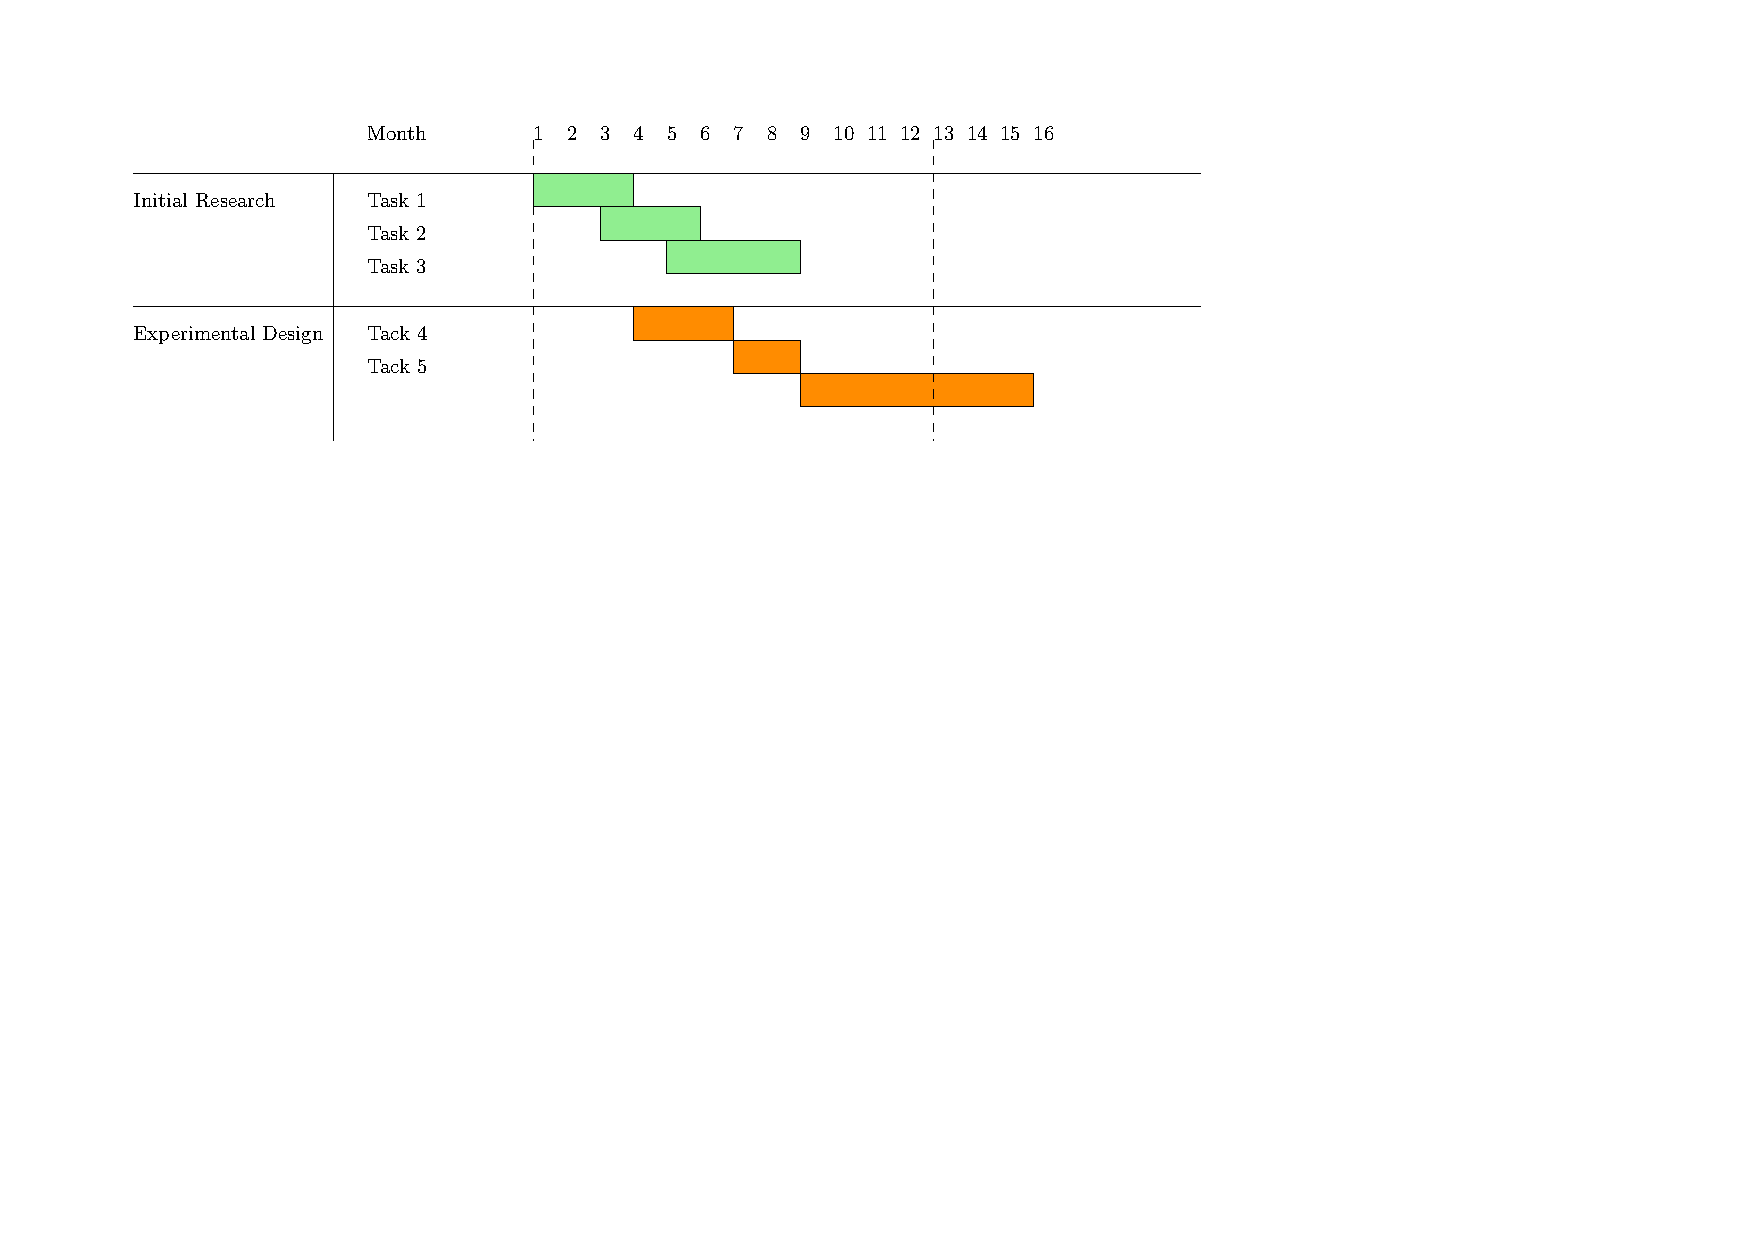
\includegraphics[width=0.7\linewidth]{images/ExampleGannt.pdf}
\caption{Gantt Chart showing timeline for planned tasks. You may edit this diagram by downloading the PDF and opening in IPE (\url{https://ipe.otfried.org}) a free Latex compatible diagram editor.\label{fig:Gantt}}
\end{figure}
\end{landscape}


\clearpage
\bibliographystyle{plainurl}
\bibliography{references}

\end{document}
